\section{Analisi Prestazionale}
Costruite le pipelines, a partire da ognuna di esse è stato addestrato un modello utilizzando il metodo \verb|.fit()|:
\begin{center}
    \verb|pipelineModel = pipeline.fit(train_data)|
\end{center}
Una volta pronto il modello, è stato testato utilizzando il metodo \verb|.transform()|. Facendo ciò, viene generato un nuovo DataFrame aggiungendo a quello di partenza una colonna con le previsioni fatte dal modello:
\begin{center}
    \verb|predictions = pipelineModel.transform(test_data)|
\end{center}
Utilizzando i modelli addestrati, sono state svolte due tipi di valutazioni. La prima tiene conto dell'accuratezza delle predizioni ottenute dai modelli utilizzando i dataset di test descritti nelle sezioni \ref{textc_data}, \ref{ner_eng_data} e \ref{ner_ita_data}. La seconda misura i tempi di esecuzione ottenuti parallelizzando il lavoro ed opera su di un dataset di 760.000 record.
\subsection{Metriche} \label{metriche}
A partire dalle previsioni prodotte, è stato generato un \textit{classification report}. Si tratta di un rapporto che descrive varie metriche relative a quanto bene ha funzionato un modello di machine learning e che si ottengono confrontando i risultati prodotti dal modello con quelli attesi. Il report mostra le principali metriche di classificazione:
\begin{itemize}
    \item \textbf{Precisione (Precision)}: la capacità di un classificatore di identificare solo le istanze corrette per ogni classe.
    \item \textbf{Richiamo (Recall)}: la capacità di un classificatore di trovare tutte le istanze corrette per una classe.
    \item \textbf{F1-Score}: media armonica ponderata di precisione e richiamo normalizzata tra 0 e 1. Un punteggio F di 1 indica un equilibrio perfetto, poiché precisione e richiamo sono inversamente correlati.
    \item \textbf{Accuratezza (Accuracy)}: valore che indica quanto spesso ci si può aspettare che il modello di machine learning preveda correttamente un risultato sul numero totale di volte che ha fatto previsioni.
    \item \textbf{Support}: numero di occorrenze effettive di una classe nel dataset.
\end{itemize}
Per i due task sono state utilizzate due tipi di valutazione differenti:
\begin{itemize}
    \item \textbf{Text Classification}: per questo task è stata scelta una valutazione rigida. Per ogni testo presente nel dataset, se la previsione del modello corrisponde al valore atteso, allora viene valutato come corretto, altrimenti come incorretto. Pertanto, il valore a cui si fa riferimento è l'accuratezza, che si calcola come il rapporto tra le predizioni corrette ed il numero di esempi totali.
    
    \item \textbf{Named Entity Recognition}: per il NER, si prende come riferimento la valutazione proposta nel task CoNLL-2003\footnote{CoNLL-2003 Paper: \href{https://aclanthology.org/W03-0419.pdf}{https://aclanthology.org/W03-0419.pdf}} e nello script \textit{conlevall}\footnote{conlleval script in perl: \href{https://www.clips.uantwerpen.be/conll2000/chunking/conlleval.txt}{https://www.clips.uantwerpen.be/conll2000/chunking/conlleval.txt}}.Le prestazioni dei sistemi sono misurate in termini di precisione, richiamo e f1-score, dove:\\
    \textit{"La precisione è la percentuale di named entities trovate dal sistema di apprendimento che sono corrette. Recall è la percentuale di entità presenti nel corpus che vengono trovate dal sistema. Una named entity è corretta solo se c'è una corrispondenza esatta dell'entità corrispondente nel file di dati".}\\
    Pertanto, il calcolo non tiene in considerazione le previsioni del tag \textit{'O'} (ovvero, chunk che non è una named entity) che sono invece valutate dall'accuracy.
\end{itemize}
\newpage
\subsection{Performance}
\renewcommand{\arraystretch}{2}
% -----------------
%  Text Classification - Inglese
% -----------------
\subsubsection{Text Classification - Inglese}
\begin{table}[hbt!]
    \centering
    \begin{tabular}{|c|c|}
      \hline
          Embedding & Accuracy  \\
      \hline
             USE    &   89\%    \\
      \hline
        Sentence BERT (base\_case)    &   89\%   \\
      \hline
    \end{tabular}
    
    \caption{Risultati per Text Classification}
    \label{tab:textc_results}
\end{table}

\begin{figure}[ht!]
    \centering
    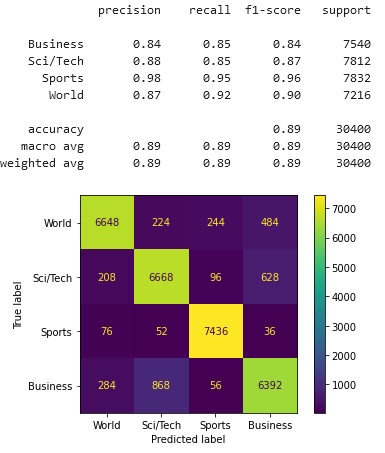
\includegraphics[width=0.7\textwidth]{img/results/cmatrix_textc_use.png}
    \caption{Text Classification - USE: classification report}
    \label{fig:creport_textc_use}
\end{figure}
\begin{figure}[ht!]
    \centering
    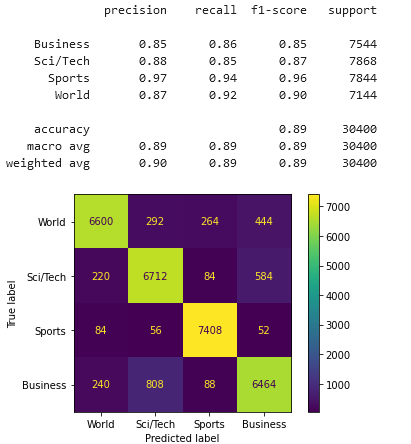
\includegraphics[width=0.7\textwidth]{img/results/cmatrix_textc_bert.png}
    \caption{Text Classification - BERT: classification report}
    \label{fig:creport_textc_bert}
\end{figure}

% -----------------
%  Named Entity Recognition - Inglese
% -----------------
\clearpage
\subsubsection{Named Entity Recognition - Inglese}
\begin{table}[ht!]
    \centering

    \begin{tabular}{|c|c|}
      \hline
        Embedding & F1-Score \\
      \hline
          GloVe  &   85.8\% \\
      \hline
          BERT (base\_case)   &   86.5\% \\
      \hline
    \end{tabular}
    \caption{Risultati per NER in Inglese}
    \label{tab:ner_eng_results}
\end{table}
\begin{figure}[hbt!]
    \centering
    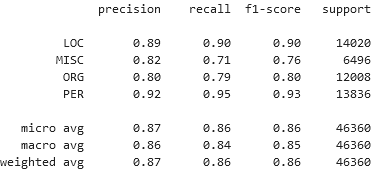
\includegraphics[width=0.7\textwidth]{img/results/creport_ner_eng_glove.png}
    \caption{NER in Inglese - GloVe: classification report}
    \label{fig:creport_ner_eng_glove}
\end{figure}
\begin{figure}[ht!]
    \centering
    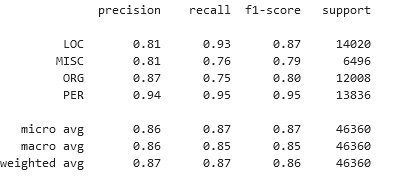
\includegraphics[width=0.7\textwidth]{img/results/creport_ner_eng_bert.png}
    \caption{NER in Inglese - BERT: classification report}
    \label{fig:creport_ner_eng_bert}
\end{figure}

% -----------------
%  Named Entity Recognition - Italiano
% -----------------
\clearpage
\subsubsection{Named Entity Recognition - Italiano}
\begin{table}[hbt!]
    \centering

    \begin{tabular}{|c|c|}
      \hline
        Embedding & F1-Score \\
      \hline
          GloVe  &   65\% \\
      \hline
          BERT (base\_case)  &   60.5\% \\
      \hline
    \end{tabular}
    \caption{Risultati per NER in Inglese}
    \label{tab:ner_ita_results}
\end{table}
\begin{figure}[hbt!]
    \centering
    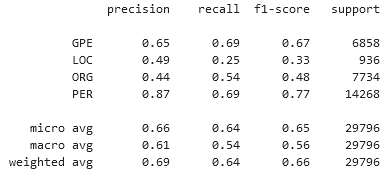
\includegraphics[width=0.7\textwidth]{img/results/creport_ner_ita_glove.png}
    \caption{NER in Italiano - GloVe: classification report}
    \label{fig:creport_ner_ita_glove}
\end{figure}
\begin{figure}[hbt!]
    \centering
    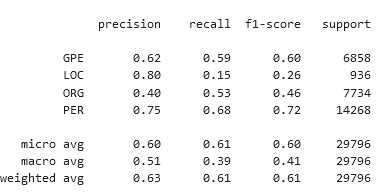
\includegraphics[width=0.7\textwidth]{img/results/creport_ner_ita_bert.png}
    \caption{NER in Italiano - BERT: classification report}
    \label{fig:creport_ner_ita_bert}
\end{figure}
\clearpage
\subsection{Tempi di esecuzione}
\begin{table}[ht!]
    \centering
    \begin{tabular}{|c|c|c|}
        \hline
            Embedding & Esecutori & Tempo di esecuzione     \\
        \hline
            \multirow{2}*{USE} &     1     &  8min 05s      \\
            \cline{2-3}        &     2     &  4min 21s      \\
        \hline
            %\multirow{2}*{Sentence BERT (base\_case)} &     1     &  8h 6min 03s  \\
            \multirow{2}*{BERT (base\_case)} &     1     &  8h 6min 03s  \\
            \cline{2-3}         &     2     &  4h 6min 05s  \\
        \hline
    \end{tabular}
    %\caption{Text Classification - Tempi di esecuzione}
    \caption{Tempi di esecuzione}
    \label{tab:execution_time}
\end{table}

% \begin{table}[ht!]
%     \centering
%     \begin{tabular}{|c|c|c|}
%         \hline
%             Embedding & Esecutori & Tempo di esecuzione     \\
%         \hline
%             \multirow{2}*{GloVe} &     1     &  ???      \\
%             \cline{2-3}          &     2     &  ???      \\
%         \hline
%             \multirow{2}*{BERT} &     1     &  ???  \\
%             \cline{2-3}         &     2     &  ???  \\
%         \hline
%     \end{tabular}
%     \caption{Named Entity Recognition - Tempi di esecuzione}
%     \label{tab:execution_time}
% \end{table}
\subsection{Valutazioni}
Nel caso del task di Named Entity Recognition, i risultati presentano una notevole differenza tra le performance ottenute con i dataset in lingua inglese e in lingua italiana. Infatti, si passa da un F1-score dell'87\% con BERT Base nel primo caso, ad un 60\% con il modello corrispettivo per la lingua italiana. Il risultato per l'inglese non raggiunge lo stato dell'arte\footnote{Risultati CoNLL 2003 (English): \href{https://paperswithcode.com/sota/named-entity-recognition-ner-on-conll-2003}{https://paperswithcode.com/sota/named-entity-recognition-ner-on-conll-2003}}, ma non si distacca eccessivamente dalle altre soluzioni al momento disponibili. Drastico è il calo che si ha con la lingua italiana, dove il modello sbaglia eccessivamente. Da quanto si evince dei risultati mostrati sul sito di \textit{evalita}\footnote{Risultati evalita 2009: \href{https://www.evalita.it/evalita-2009/results/}{https://www.evalita.it/evalita-2009/results/}}, le soluzioni per questo task raggiungono anche valori di F1-score pari all'82\%, ovvero circa il 20\% in più del modello studiato in questa tesi. I risultati peggiori, come si legge dal classification report, si incontrano nei casi dei tag che identificano \textit{entità geo-politiche (GPE)} e \textit{organizzazioni (ORG)}.
\begin{figure}[ht!]
    \centering
    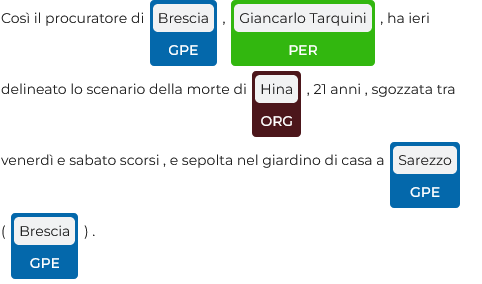
\includegraphics[width=0.8\textwidth]{img/errori_ner_ita/errore1.png}
    \caption{Named Entity Recognition per l'italiano - Errore 1}
    \label{fig:ner_errore1}
\end{figure}
\begin{figure}[ht!]
    \centering
    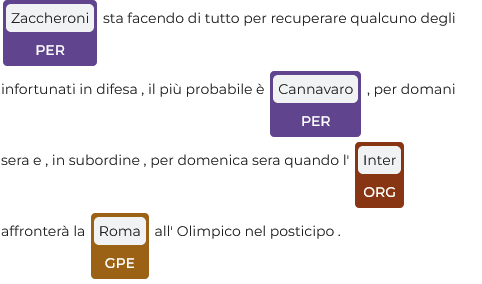
\includegraphics[width=0.8\textwidth]{img/errori_ner_ita/errore2.png}
    \caption{Named Entity Recognition per l'italiano - Errore 2}
    \label{fig:ner_errore2}
\end{figure} \newpage
Osservando la figura \ref{fig:ner_errore1}, si nota come nomi poco frequenti in Italia (in questo caso \textit{Hina}), non vengono interpretati come riferimenti a persone, ma ad altre entità (in questo caso \textit{organizzazione (ORG)}).
Inoltre, il modello fatica a distinguere le ambiguità che si presentano quando un'entità che solitamente è utilizzata con un significato, si presenta nella frase con un'altra accezione. Facendo riferimento all'immagine \ref{fig:ner_errore2}, il concetto di \textit{Roma} come associazione sportiva, e quindi \textit{organizzazione}, viene confuso con il significato di \textit{Roma} intesa come la città capitale d'Italia. La parola è stata pertanto classificata come entità \textit{geo-politica}.
 

Un'ulteriore differenza tra i dati ottenuti dai due dataset, si ha con l'accuratezza raggiunta dai modelli. Anche se di poco, BERT performa meglio di GloVe nella lingua inglese (86.5\% il primo, 85,8\% il secondo), mentre per la lingua italiana, GloVe riconosce leggermente meglio le ambiguità rispetto alla controparte (65\% per GloVe, 60,5\% BERT).\\
\\
Passando al problema di Text Classification, sia il componente UniversalSentenceEncoder sia il BertSentenceEmbedding, riportano ottimi risultati in termini di accuratezza, raggiungendo entrambi l'89\%. La differenza sostanziale si nota nei tempi di esecuzione, nei quali l'\verb|UniversalSentenceEncoder| risulta essere decine di volte più veloce. Pertanto, a parità di risultati, USE è l'alternativa che offre il miglior rapporto tra l'accuracy e i tempi di esecuzione sui dataset utilizzati.\\
\\
É facilmente osservabile che, all'aumentare della dimensione del sistema distribuito, e quindi degli esecutori, Spark NLP migliora di gran lunga le sue prestazioni. La differenza si nota in particolar modo con BERT, dove non si ottiene ancora un risultato in tempi competitivi ma, con l'aggiunta di un nodo worker, il tempo di esecuzione si dimezza. Questo denota una buona distribuzione del carico di lavoro tra i nodi dovuta ad un'equa suddivisione dei jobs tra i vari esecutori. 

In sistemi che utilizzano frequentemente centinaia se non migliaia di nodi, Spark NLP può offrire predizioni accurate in tempi contenuti.